%----------------------------------------------------------------------------------------
%	INTRODUCTION
%----------------------------------------------------------------------------------------
\section{Introduction}

An essential step in the commercial asparagus cultivation is the sorting of the harvested stalks into different quality classes. Depending on size, shape and colour, a label is assigned to the individual spears which determines the class of the asparagus. Nowadays, this task is usually performed automatically, with modern asparagus sorting machines achieving a throughput of up to twelve spears per second (\url{https://www.heringinternational.com/fileadmin/media/archive1/downloads/presseberichte/2015-09-23\textunderscore FAZ\textunderscore -\textunderscore Verlagsspezial\textunderscore Industrierregion\textunderscore S\%C3\%BCdwestfalen\textunderscore -\textunderscore Textilbeton\textunderscore f\%C3\%BCr\textunderscore Dior.pdf}). However, the accuracy of such machines can be unsatisfying. Manual resorting is usually necessary, and thereby causes substantial effort. \\
\\
The aim of this study project was to investigate how techniques from computer vision, both classical and deep learning based, can be applied to improve classification results for the asparagus sorting machines. The metric for the sorting corresponds to the quality of an asparagus. The quality in turn is defined based on a number of features that represent differences (or even flaws) in colour, shape, or texture. Hence, improving sorting algorithms for the classification of asparagus requires reliable means of measuring these features. As such, we were interested in the question how the quality-defining features of asparagus spears can be estimated using state of the art computer vision and machine learning techniques. \\
Besides the systematic engagement with feature detection methods from the field of machine learning, the study project was also used as a training ground for project management. The hands-on experience on a long-term project gave the chance to learn how to distribute work and how to organize ourselves in a larger team. \\
The project was supported by a local asparagus farm and a company specializing in asparagus sorting machines. They provided training data and expertise on the classification of the spears. The idea to apply new machine learning approaches to a commercial problem of the agricultural industry seemed promising and challenging at the same time. As the data received from the farm was unlabelled, a larger focus on the preprocessing of the recorded image data became inevitable. Further, the variance in quality classes and the subjective view of human sorting behaviour toughened the perspective on a practical application into the actual sorting machine. Nevertheless, the original goal of studying different techniques in computer vision and testing their usability in a restricted hardware setting for asparagus classification gave valuable insights into the practical application of previously only theoretically assessed knowledge. \\
Over the course of one year, the team members worked on the implementation of different approaches to tackle the issue of image classification. After intense engagement with the subject, the methodologies and the project outcome were documented and critically reviewed. On the following pages, the different stages of the project together with the results of the applied computer vision approaches are described in detail. The report chapters are mostly in chronological order, each with the focus on a different stage of the study project throughout the year. \\
\\
In the first chapter, the idea of the project is presented together with an introduction to the current standards of image classification in machine learning as well as a general background on the quality classes, the sorting process, and classification of asparagus in the agricultural industry. Further, the results of the project are summarized in short at the end of the chapter, to provide a comparison of the expected outcome at the start of the project with the results that were achieved after the year. \\
The second chapter comprises the organizational background to the project. This includes task management and teamwork, as well as a thorough evaluation of our planning abilities as a group. Further, the process of data collection and a first inspection of the sorting machine are elaborated, with an emphasis on the first issues of unlabelled data. Unfortunately, the research for scientific literature, specifically regarding our topic of agricultural application of deep learning approaches, proved mostly disappointing. Nevertheless, it gave an insight into practical possibilities and a rough guideline for our endeavour. The collected literature that was found to be close to our topic is reported at the end of the second chapter. \\
In the third chapter, the preprocessing phase is captured with the building of the data set at its end section. The first classical machine learning techniques for automatic feature extraction on image data are explored, followed by the process of manual feature extraction with the usage of a labelling application. The resulting outcome is reported, evaluated, and the labelled image data is transformed into a data set for the further training of the chosen models. \\
The fourth chapter constitutes the different approaches that were chosen to tackle the issue of image classification. An emphasis was put on the application of deep learning techniques for the classification of the asparagus. As the collected data includes labelled and unlabelled samples, methods from the range of supervised learning to unsupervised learning were tested. \\
The fifth chapter contains the results of the project. The outcome of each approach is described and compared to other methods as well as to the original classification accuracy of the sorting machine at the asparagus farm. Further, all approaches are critically reviewed and discussed with an evaluation of their practical application in the food industry. The overall outcome of the project is judged as a scientific study and as a team management experience. \\
In the sixth chapter our findings are set into a broader perspective. The project and its results are summarized on a scientific basis as well as on the organizational level while future prospects of the project are assessed. \\
 \\
Before delving any deeper into the specific context of software development for the application in classification tasks, however, a thorough insight into the idea of the study project is given in the following chapter. Further, a rough background on the addressed topics of machine learning and the sorting of asparagus are provided.
In 1.1 \textit{The project}, the objective of the study project is introduced. The next section, 1.2 \textit{Background on computer vision-based classification tasks}, gives an overview on the machine learning techniques that explore how image classification can be implemented and how these approaches can provide a solution to our issue. In 1.3 \textit{Background on sorting asparagus}, the process of asparagus classification in the commercial food industry is illustrated and the different quality classes of asparagus are defined. The first chapter concludes with 1.4 \textit{Expected outcome vs actual outcome}, where the results of the study project are presented on a broad level and compared to the expected outcome.


\subsection{The project}

The objective of the study project was to find both, conventional and neurally-inspired computer vision based approaches which can be tested for their practical application in the commercial sorting of white asparagus. The different methods were implemented based on the image data that was received from the automatic sorting machine Autoselect ATS II employed by the asparagus farm “Gut Holsterfeld”. The aim was to check whether approaches from the fields of machine learning and computer vision can be applied to improve the classification behaviour of the asparagus sorting machine and, thus, if they can be used in a more industrial than scientific setting regarding the specific problem of asparagus classification. The initial intention to directly implement new software into the machine was put in the back to make room for intensive research on the different approaches and on fine-tuning the received data to build a practical data set to train neural networks.
The idea for the project was formed by one of the students of the study group. She was in contact with the asparagus farm “Gut Holsterfeld” and had received note of the unsatisfying classification performance of its sorting machine. The practical application to a real world problem sparked the interest of the group and the general curiosity towards computer vision, in particular neural networks, further inspired to deal with the sorting issue in a deep learning context. \\
All project members were students in the field of Cognitive Science at the University of Osnabrück. The study project is part of the Master Program in Cognitive Science at the University of Osnabrück. It was supervised by Dr. Ulf Krumnack (\url{https://www.ikw.uni-osnabrueck.de/en/research\textunderscore groups/computer\textunderscore vision/people/krumnack_ulf.html}) and Axel Schaffland, M.Sc. (\url{https://www.ikw.uni-osnabrueck.de/en/research\textunderscore groups/computer\textunderscore vision/people/schaffland\textunderscore axel.html}). \\
The intention of the study project is to confirm the ability of its participants to independently formulate and solve an unknown problem from the scientific context of one subject area using the methods and terms of a previously theoretically learned subject~\citep{studyregulations}~\citep{moduledescription}. This includes the documentation and presentation of the results, the methodologies as well as the reflection on the work process. Within the scope of the project, for example, the development of software, analysis and interpretation of statistical data material are practiced. A further aspect of the study project is to deepen the communicative and decision-making competence of its participants~\citep{moduledescription}. The idea is to train independent project work in groups of students under conditions that are common for research projects in science or industry. \\
As the project took part in the scope of an examination for the Cognitive Science master program at the University of Osnabrück, most of the work was developed at the university, that is, at the Institut für Kognitionswissenschaften (IKW).
The project was realized as a cooperation with a local asparagus farm “Gut Holsterfeld”, at Rheine (\url{https://www.gut-holsterfeld.de/}). Additional image data was received from the asparagus farm Querdel (\url{https://www.querdel.de/}). Further cooperation existed with the mechanical engineering company HMF Hermeler Maschinenbau GmbH (\url{www.hmf-hermeler.de}) that developed the sorting machine Autoselect and provided valuable expertise on the sorting issue. \\
The documentation to the project can be found at (\url{https://asparagus.readthedocs.io/en/latest/}), all associated software is stored in the Github repository CogSciUOS/asparagus (\url{https://github.com/CogSciUOS/asparagus}) and at the institute internal storing system (PATH). \\
\\
In the next section, an introduction to the field of computer vision based approaches for the classification of data is given. It provides a theoretical background on the broad selection of different techniques that can deal with the objective of this project, namely the improvement of sorting commercial asparagus into quality classes with a machine.



\subsection{Background on computer vision based classification tasks}

In the following chapter, we are going to describe the current standard of computer-based image classification. Our main focus will be on artificial neural networks and classical computer vision techniques. We will give a broad overview of relevant topics and underline their importance for our project. Computer vision is a field of computer science that aims to automatically extract high-level understanding from image data and provide appropriate output. It is closely linked with machine learning, which describes the ability of a system to learn and improve from experience rather than being specifically programmed. Machine learning is frequently used to solve computer vision tasks. \\
\\
Image classification is one of the main subfields of computer vision which gained a lot of attention in the scientific as well as the economic world. Besides the classical computer vision techniques that use algorithmic approaches to determine patterns, edges, and other points of interest that can help to classify images, artificial intelligence was introduced to the field in the 1960s. Since then, more and more creative and complex artificial neural networks were introduced to solve numerous classification tasks including letter, face, and street sign recognition among others~\citep{mironczuk2018recent} ~\citep{balaban2015deep} ~\citep{stallkamp2011german}. \\
Some experts in the field claim that artificial neural networks revolutionized the field of image classification, yielding better results than ever before~\citep{he2016deep} ~\citep{krizhevsky2012imagenet}. More and more challenges, for example ImageNet, were introduced and computer scientists all over the world implemented creative solutions for the proposed problems. Additionally, influential companies like Google had a deep interest in finding solutions for image-based classification problems and pushed the research on this and related topics even further. In the era of optimization, computer-based classification became indispensable in many industries and also found its way into agriculture which is the field of interest in this study project.
In the following, a short introduction in both classical computer vision techniques and artificial neural networks is given which will span a bridge to our current classification problem. \\
\\
Neural networks are used for image classification in many domains. In contrast to the algorithmic approaches, it is not determined by the programmer how and what exactly the model learns. A large amount of data is provided to the model, which then extracts relevant information to learn the classification task. But what is relevant to the model is not necessarily relevant or interpretable to a human observer. This is one of the biggest disadvantages compared to the classical computer vision approaches, which are understandable and, therefore, interpretable and adjustable. Another problem that comes along with this is that the bias for those approaches often does not lie in the code itself but in the data, which is by far more difficult to detect and surpass. For this reason, many see artificial neural networks as a black box, which may yield great results but can never be fully understood. Recent advances try to tackle that issue by researching artificial intelligence systematically aiming at making it explainable~\citep{tjoa2019survey}~\citep{gilpin2018explaining}. \\
In image classification, usually convolutional neural networks (CNNs) are used, which are inspired by the visual cortex of the brain. The idea is that highly specialized components or, in the case of CNNs, filters learn a very specific task, which is similar to the receptive fields of neurons in the visual cortex~\citep{hubel1962receptive}. These components can then be combined to high-level features, which can then in turn be combined to objects that can be used for classification. In CNNs this concept is implemented by several successive convolutional layers in which one or more filters are slid over the input generating so-called feature maps. Each unit in one feature map looks for the same feature but in different locations of the input. In recent years, CNNs became so good that they outperform humans in many classification tasks~\citep{russakovsky2015imagenet}(\url{http://karpathy.github.io/2014/09/02/what-i-learned-from-competing-against-a-convnet-on-imagenet/}). \\
\\
Although machine learning exhibits very promising results and a lot of research and literature is available on the topic, many branches of industry still rely on traditional computer vision techniques in their implementation of image classification. This also applies to the asparagus sorting paradigm. To the best of our knowledge, no asparagus sorting machine is currently on the market that uses artificial intelligence for its classification algorithm. This brings us to the second topic of this chapter, namely the classical computer vision algorithms. \\
Many classical computer vision algorithms aim to detect and describe points of interest in the input images that can be generalized to features. For these features, low-level attributes such as rapid changes in colour or luminance can be used. In contrast to the features learned with the help of machine learning, these features are not specific to the training data set and therefore do not depend on it being well-constructed. Further, they are usually created in a way that is interpretable by humans which makes them very flexible and easily adaptable to specific use cases. This is why in some cases, traditional computer vision techniques can solve a  problem much more efficiently and in fewer lines of code than machine learning approaches. \\
\\
In summary, both approaches have interesting implications for computer-based image classification tasks and provide us with promising techniques for our problem of asparagus classification. While we relied mostly on machine learning for the classification task itself, traditional computer vision algorithms were used to detect important features from the images, which not only helped us in the labelling process but also can be used for some of the binary classification tasks of the hand-labelled features.


\subsection{Background on sorting asparagus}

In this section, the different sorting classes for asparagus are discussed with a focus on the classification of the 13 quality classes as characterized by the asparagus farm “Gut Holsterfeld” and implemented for our project aim. Two additional sources of information for the following issue were the owner of the asparagus farm “Gut holsterfeld”, Mr. Silvan Schulze-Weddige, and the CEO of the engineering company “HMF Hermeler Maschinenbau”, Mr. Thomas Hermeler. \\
\\
While asparagus accounts for a fifth of the area used for vegetable cultivation in Germany, the harvesting season of white asparagus only spans over a period of 2 months, beginning in April and usually ending on the 24th of June ~\citep{spargelstatistik} ~\citep{nrw2018spargel}. During this period, the asparagus is harvested, classified, and sold in accord with a price range that is defined by the quality class of the asparagus. \\
In the European Union, there is a uniform system for the sorting of asparagus into quality classes~\citep{euspargelnorm} ~\citep{unspargelnorm} (\url{https://mlr.baden-wuerttemberg.de/de/unser-service/presse-und-oeffentlichkeitsarbeit/pressemitteilung/pid/nationale-handelsklassen-fuer-frisches-obst-und-gemuese-abgeschafft-1/})(\url{https://www.bzfe.de/inhalt/spargel-kennzeichnung-5876.html}). However, supply and demand usually determine the number and accuracy of these categories. One of the first defining features is the colour of the asparagus which comprises four categories: white, violet, violet-green, and green~\citep{euspargelnorm}. For this project, only the first two colours were of relevance. Further distinction is made between class Extra, class I, and class II, where the class Extra defines the product as perfect quality, class I defines it as good quality, and class II includes products that do not qualify for the other classes but satisfy the minimum requirements for commercial distribution~\citep{euspargelnorm}. A last distinction is made in the characteristics length and width. White and violet asparagus may not exceed 22 cm in length. The minimal length of the spear is above 17 cm for long asparagus, 12-17 cm for short asparagus, 12 cm for class II, and less than 12 cm for fractured spears with intact heads. Additionally, there is some level of tolerance accepted for the quality classes. In class Extra, 5\% of class I asparagus is tolerated. Class I allows for 10\% wrongly sorted asparagus of class II. In class II 10\% of spears are accepted that do not suffice for the minimum requirements of asparagus trade. The last quality difference that has to be fulfilled on a national basis is that there are no more than 15\% of hollow spears tolerated in one package or bundle. \\
Depending on how carefully the individual farmer further categorizes the asparagus, additional classes can be established. Regional differences to those classes make the challenge for the manufacturers of sorting machines even more complicated. The classes as stated in this report depend solely on the views of the farm Gut Holsterfeld and do not necessarily apply to any other classification system of the asparagus industry. \\
In the Table ~\ref{tab:AsparagusLabels}, 14 quality classes are shortly described, of which 13 classes were relevant to this project. The classification tree in Fig~\ref{fig:LabelTree} illustrates the decision process that underlies the categorization of the relevant 13 asparagus classes.

\begin{table}[H]
	\centering
	\begin{tabular}{l p{11cm}}
		\textbf{Label} & \textbf{Description} \\
		\noalign{\smallskip}
		\hline
		\\
		I A Anna & In this context, quality class Extra is represented by I A Anna, I A 	 		Bona, and I A Clara. I A is defined as asparagus that is perfectly straight and 		 		white. There are no large pressure marks, no rust, no violet colour, and no  	  	   		curvature. The identification label Anna marks that the width (diameter) of the  	 		spear is in a range of 20 to 26mm. \\
		\\
		I A Bona & Class Extra asparagus and the spear is of width 18 to 20 mm. \\
		\\
		I A Clara & Asparagus with a width of 16 to 18 mm and of quality class Extra. \\
		\\
		I A Krumme & The asparagus fulfills all criteria for class I A while it shows a 				slight curvature. \\
		\\
		I A Violett & The asparagus is of a violet complexion, while it complies with all 			guidelines for quality class I A. \\
		\\
		II A & The asparagus is both curved and violet. \\
		\\
		II B & The asparagus is curved, rusty, and/or in any other way damaged or 					classified as defective product. \\
		\\
		Rost & The asparagus shows traces of rust or has rusty parts. \\
		\\
		Dicke & The asparagus exceeds the norm of 26 mm in width. \\
		\\
		Hohle & The asparagus is hollow from the inside. \\
		\\
		Blume & The head region of the asparagus is about to bloom or it shows clear 					outlines of a flower. \\
		\\
		Suppe & The asparagus has a width of less than 16 mm. \\
		\\
		Bruch & Any asparagus that is below a length of 21 cm. However, another 						distinction in this category is made between asparagus that has an intact head and 		a length of at least 100 mm (Kerze),  an asparagus without head (Bruch), and an 				asparagus head alone (Köpfchen). \\
		\\
		Keule & The upper end of the asparagus is thicker than the lower part. The shape 				is similar to a club, hence the name of the class. This category was of no concern 		to the project because no image data of this category could be recorded. \\
		\\
		\hline
	\end{tabular}
	\caption[List of Asparagus Quality Classes]{\textbf{List of Asparagus Quality Classes}~~~In this table, 14 quality classes for asparagus categorization are listed and described, according to the asparagus farm "Gut Holsterfeld". Except for the class Keule, the 13 quality classes were used as the class label for the asparagus classification.}
	\label{tab:AsparagusLabels}
\end{table}


\begin{figure}[h]
	\centering
	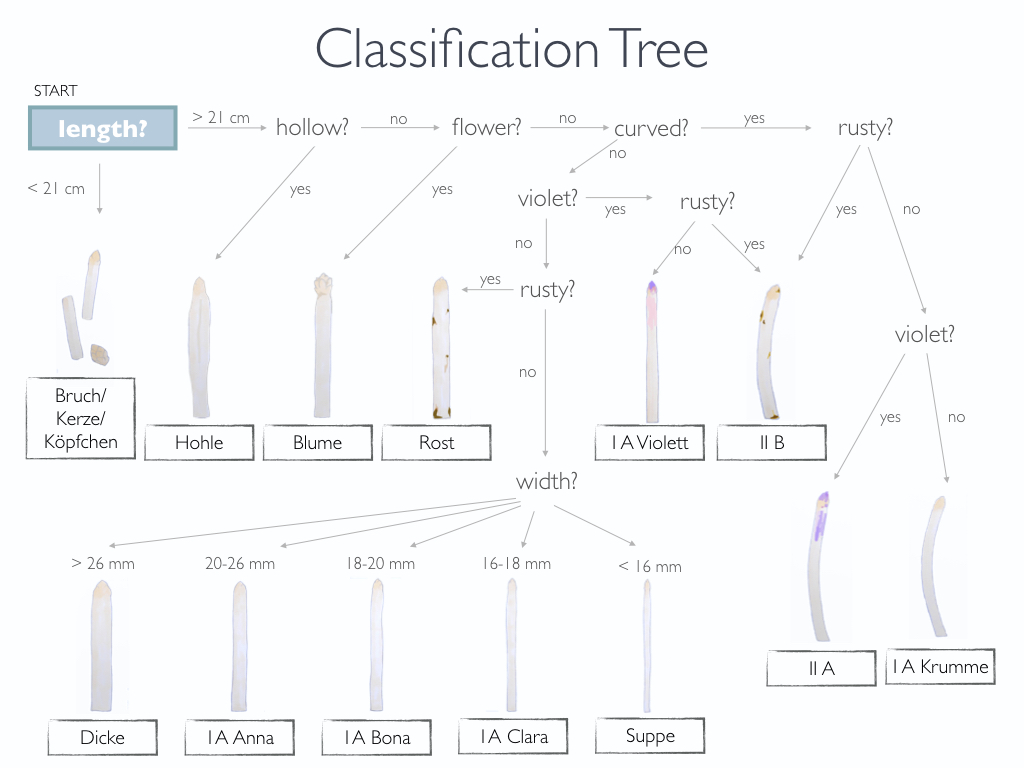
\includegraphics[scale=0.39]{Figures/chapter01/fig_tree_with_title}
	\decoRule
	\caption[Asparagus Classification Tree]{\textbf{Asparagus Classification Tree}~~~The classification tree shows how each asparagus is attributed with a label of its quality class. It follows the sorting rules of the asparagus farm “Gut Holsterfeld”. Starting from the upper left corner of the image, mostly binary decisions are made until a label is reached. The width of the asparagus is further subdivided at the end. Any further damaged or defective asparagus automatically belongs in category II B.}
	\label{fig:LabelTree}
\end{figure}

One of the challenges of asparagus classification with a machine lies in the human sorting error. While the human sorter can distinguish between colours or between shapes like bent or flowering, a machine works even more precisely. The machine can assess exact calculations about the length or the width of a spear. Thus, a threshold has to be defined if a spear is sorted into a certain class. However, the data on which the machine calculates its features to characterize an asparagus spear was previously labelled by a human. The subtle differences in colour might have escaped the sorter and hence the machine will sort a spear into the category Rost while the spear would be judged as category I A Anna by the human sorter. Since the human sorting behaviour is subjective, the same asparagus can be categorized differently by two independent sorters. Furthermore, an asparagus sorted twice by the same person at different points in time might not end up in the same category than before. \\
A second problem for the sorting machine poses the distinction between different colours. The machine might not be able to distinguish whether the asparagus was, e.g. very rusty or simply very dirty in certain cases. \\
A third factor for classification difficulties is caused by the restricted view of the product. An asparagus can look perfectly shaped from one angle but might be damaged on the side that is not exposed to the camera of the sorting machine. \\
Another complication poses the question of demand and supply. During some seasons there is more asparagus of a certain class and less of another class is available. The farmer usually arranges the number of spears belonging to a quality class according to the seasonal conditions. For example, during a season with less high quality asparagus of classes I A, the sorting threshold will shift. Spears that are usually sorted into, e.g. a lower class will now belong to a higher class. The machine has to be flexible to accord for this change of preferences. \\
These challenges are not impossible to overcome but they make it more difficult to find a solution to the sorting task and compromises might be necessary. \\
\\
To summarize this subchapter, there are 13 quality classes of asparagus relevant for this project. The spears are labelled according to features that influence the price of a spear. Further, the challenge for a sorting machine will not only be to sort for these criteria but to provide a flexible and individual solution in accord with the farmer.


\subsection{Expected outcome vs. actual outcome of the project}

Based on the literature review, we aimed to improve the current sorting performance of the ATS II machine at the local asparagus farm “Spargelhof Gut Holsterfeld”. In this report, we investigated techniques from computer vision, both classical and deep learning based approaches. We expected to reach a result which is able to classify asparagus images into 13 different classes better than the current standard. For the initial performance of the sorting machine, no reliable accuracy of correctly sorted asparagus pieces is available, but between three and six workers are employed to re-sort wrongly classified asparagus pieces. The farmer himself assumes an accuracy of not more than 70\%. \\
 
An advantage of our project is that it was directly supported by the local asparagus farm, providing training data and allowing us to evaluate our proposed solutions in a real environment during the asparagus harvesting season 2020. \\
\\
However, there was a misunderstanding between us and the supporting asparagus farm about the kind of data we need. The existing images were too few, and also unlabelled. Therefore, we spent the first two and a half months with data acquisition instead of starting with preprocessing as we originally planned. Throughout the harvesting season 2019, we continuously went to the asparagus farm and collected unlabelled asparagus images during the normal harvesting procedure (see also 2.3). For 12.962 images (for more detail see 2.3), we collected labelled data by taking images of pre-sorted asparagus pieces. Pre-sorted in this context means that the asparagus pieces were sorted by the sorting machine and if needed re-sorted manually by professional workers. We would have wanted to collect more data this way, but this was not possible, as the asparagus quality suffered from it (for more detail see 2.3). \\
The number of labelled images is insufficient to learn classes using deep learning approaches~\citep{russakovsky2013detecting}~\citep{russakovsky2010attribute} (\url{https://petewarden.com/2017/12/14/how-many-images-do-you-need-to-train-a-neural-network/}). Therefore, we spent six months preprocessing and labelling the data manually. Preprocessing involved: organizing the large number of images, renaming the files, so that the three images of one asparagus piece can be accessed together, and performing automatic feature extractions (ref to preprocessing).To label the images by hand, we wrote a custom application (reference hand-label-assistant). The final labelled data set contains over 10.000 (13.319) labelled asparagus pieces. Next, we worked on numerous classical and deep learning approaches (ref to chap 4). We reached several very interesting results which will be discussed in Chapter 4. Although we developed an end-to-end prototype, we did not deploy it onto the sorting machine for the harvesting season 2020. Even though some of our results are highly promising, it is therefore difficult to compare it to the current performance of the machine. \\
 \\
\textit{Hier noch ein Absatz mit den Inhalten aus der Conclusion – sobald diese steht.} 

